\chapter{Electrical \& Fluid Connectors}\label{ch:connectors}

\begin{tipbox}[When to Read This Chapter]
\textbf{Sprint~3 (CDR)}: Read when selecting connectors for your BOM. Focus on the connector family quick-reference table and the selection framework. \textbf{Sprint~4--5}: Return to the failure modes section (fretting corrosion, contact resistance) when debugging intermittent connections. \textbf{Fluid projects}: Read the NPT vs.\\ BSP section before ordering any fittings.
\end{tipbox}


\begin{tipbox}[When to Consult This Chapter]
\textbf{Sprint~3 (CDR)}: When specifying connectors in your BOM and wiring diagrams. Use the quick-reference table at the end for common families. \textbf{Sprint~4--5}: When debugging intermittent connections during integration.
\end{tipbox}

% ── Title Block ───────────────────────────────────────────────────────


\vspace{1em}

% ── Learning Outcomes ─────────────────────────────────────────────────



\vspace{1em}

% ══════════════════════════════════════════════════════════════════════
\section{Electrical Connectors}
% ══════════════════════════════════════════════════════════════════════

\subsection{Connector Anatomy}

Every electrical connector consists of three fundamental elements:

\begin{enumerate}[leftmargin=1.5em]
  \item \textbf{Contacts}. The conductive pins (male) and sockets (female) that carry electrical current. Typical base metals are phosphor bronze and beryllium copper (BeCu), plated with either gold (best corrosion resistance, lowest contact resistance) or tin (lower cost, adequate for benign environments).

  \item \textbf{Housing}. The insulating body that mechanically positions and electrically isolates the contacts. Common housing materials include:
  \begin{itemize}[nosep]
    \item Nylon (PA66); general purpose, good toughness, low cost.
    \item PBT (polybutylene terephthalate); higher stiffness, better chemical resistance.
    \item LCP (liquid crystal polymer); highest temperature rating, used in reflow-soldered connectors.
  \end{itemize}

  \item \textbf{Termination}. The mechanical and electrical joint between the wire conductor and the contact. The five major termination methods are detailed in Section~\ref{sec:termination}.
\end{enumerate}

\subsection{Gender Convention}

\begin{itemize}[leftmargin=1.5em]
  \item \textbf{Male} (plug/header): pins protrude from the connector face.
  \item \textbf{Female} (receptacle/socket): pins are received into sockets.
  \item In wire-to-wire assemblies, one cable carries the plug, the other the receptacle.
  \item In wire-to-board applications, the board-mounted header is typically male.
\end{itemize}

\subsection{Keying and Polarization}

Connectors use physical features to ensure correct mating orientation and prevent damage from incorrect insertion. Common keying methods include key slots, asymmetric housing profiles, color coding, and differentiated contact arrangements.

\begin{warningbox}[Design Rule]
Always specify keyed connectors when your design has multiple similar-looking connections. Incorrect mating can destroy components, and in student projects this is one of the most common causes of electrical failure on first power-up.
\end{warningbox}


\subsection{Connection Types}

Electrical connectors are classified by \emph{what} they connect:

\begin{table}[htbp]
\centering
\small
\begin{tabularx}{\textwidth}{l X X}
  \toprule
  \textbf{Type} & \textbf{Description} & \textbf{Typical Examples} \\
  \midrule
  Wire-to-Wire & Joins two discrete wires or cable harnesses. Both sides are free-hanging connectors. &
    Molex Mini-Fit Jr., JST SM, Deutsch DT, automotive weatherpacks \\[4pt]
  Wire-to-Board & Connects a wire harness to a printed circuit board (PCB). One side is a cable connector; the other is soldered to the board. &
    JST XH/PH, Molex KK 254, pin headers with crimp\index{crimp termination} housings \\[4pt]
  Board-to-Board & Connects two PCBs directly, often in stacked or mezzanine configurations. No wires involved. &
    Board-to-board headers, mezzanine connectors, card-edge connectors \\
  \bottomrule
\end{tabularx}
\caption{Electrical connector classification by connection type.}
\end{table}

\begin{figure}[htbp]
\centering

\includegraphics[width=\textwidth]{master_figs/fig1_connector_taxonomy.png}
\caption{Electrical connector taxonomy by connection type with five termination methods.}
\label{fig:connector_taxonomy}
\end{figure}

\subsection{Harsh-Environment Connectors}

Students designing vehicle harnesses, outdoor systems, or launch hardware will encounter connectors engineered for abuse. Understanding the physical components of these systems is essential for specifying them correctly.

\textbf{Deutsch DT / DTM Series} (automotive/off-highway): These use a wedgelock that mechanically retains all contacts simultaneously, independent of the wire seal. Each cavity receives a silicone wire seal that grips the insulation OD, providing IP67/IP69K protection. Contacts are stamped-and-formed with a barrel crimp; the crimp must capture both the conductor and the insulation for strain relief. Deutsch connectors are the de facto standard for SAE Baja, Formula SAE, and agricultural equipment harnesses.

\textbf{MIL-DTL-38999 Series III} (aerospace/defense): A bayonet-coupled circular connector with a self-locking coupling ring that resists vibration. Uses machined contacts (not stamped) with interference-fit rear grommets for environmental sealing. Rated for extreme vibration (per MIL-STD-810), wide temperature ranges ($-65$ to $+200$\,\degC{}), and EMI shielding via conductive shell-to-shell contact. If your design involves launch hardware, flight systems, or classified defense work, 38999 is the starting point.

\textbf{Common to both}: Proper barrel crimps are critical; the crimp must form a gas-tight cold weld in the conductor barrel \emph{and} a secure grip in the insulation barrel. Using generic pliers instead of a calibrated ratchet tool produces crimps that look acceptable but fail under vibration or thermal cycling.


\subsection{Termination Methods}
\label{sec:termination}

The termination method is how the wire conductor is mechanically and electrically bonded to the connector contact. Each method involves different tools, skill levels, and performance characteristics.

\subsubsection{Crimp}

A precision die compresses a metal barrel around a stripped wire conductor, creating a gas-tight joint through cold-welding at the metal interface.

\begin{itemize}[nosep,leftmargin=1.5em]
  \item \textbf{Strengths}: Fast, repeatable, no heat required, excellent vibration resistance, gas-tight joint resists corrosion.
  \item \textbf{Limitations}: Requires calibrated crimp tools (hand ratchet or pneumatic); die must match the contact exactly. Poor crimps are invisible failures.
  \item \textbf{Best for}: Production wiring, automotive harnesses, harsh-environment connectors.
  \item \textbf{Quality verification}: Pull-test a sample of crimps per IPC/WHMA-A-620. Cross-section crimps periodically to verify cold-weld zone.
\end{itemize}

\begin{warningbox}[Pin Extraction: Use the Right Tool]
In prototype environments, students inevitably insert a contact into the wrong cavity. \textbf{Never} yank the wire or use a paperclip to extract a crimped pin; this damages the housing retention lance and the contact, creating an unreliable connection that will fail in service. Every connector family has a specific extraction tool (typically a thin-walled sleeve that depresses the retention lance). Keep the correct extraction tools on hand alongside your crimp tools; they cost a few dollars and save hours of rework and scrapped housings.
\end{warningbox}

\subsubsection{Solder}

Molten solder alloy (typically SAC305 lead-free or Sn63/Pb37) forms a metallurgical bond between wire and contact.

\begin{itemize}[nosep,leftmargin=1.5em]
  \item \textbf{Strengths}: Low contact resistance, well-understood process, easy visual inspection.
  \item \textbf{Limitations}: Requires heat (risk of insulation damage), not reworkable without desoldering tools, solder joints are brittle under vibration and thermal cycling.
  \item \textbf{Best for}: Board-level connections (through-hole and SMT), prototype wiring, low-vibration environments.
\end{itemize}

\subsubsection{Insulation Displacement Contact (IDC\index{IDC (insulation displacement)})}

A sharp, slotted contact blade pierces through wire insulation and makes contact with the conductor, all in a single operation.

\begin{itemize}[nosep,leftmargin=1.5em]
  \item \textbf{Strengths}: Extremely fast, no stripping required, good for mass-termination of ribbon cables.
  \item \textbf{Limitations}: Limited to small wire gauges (typically 22--28~AWG), not suitable for high-vibration environments, contact can relax over time.
  \item \textbf{Best for}: Ribbon cable connectors, low-current signal wiring, internal PCB connections.
\end{itemize}

\subsubsection{Screw Terminal}

A screw clamp compresses the wire conductor against a metal plate or barrel inside the terminal block.

\begin{itemize}[nosep,leftmargin=1.5em]
  \item \textbf{Strengths}: Tool-free or simple screwdriver, field-serviceable, wide wire gauge range, easy to inspect.
  \item \textbf{Limitations}: Bulky, screws can loosen under vibration, relatively high contact resistance compared to crimp.
  \item \textbf{Best for}: Panel-mount terminal blocks, DIN-rail wiring, power distribution, industrial controls.
\end{itemize}

\subsubsection{Press-Fit (Compliant Pin)}

A specially shaped contact pin (often an ``eye-of-needle'' or ``action pin'' geometry) is pressed into a plated through-hole on a PCB, creating a gas-tight interference fit.

\begin{itemize}[nosep,leftmargin=1.5em]
  \item \textbf{Strengths}: No solder required, excellent reliability, eliminates solder joint fatigue, good for backplane connectors.
  \item \textbf{Limitations}: Requires controlled insertion force and tooling, board must have proper hole tolerances, not field-reworkable.
  \item \textbf{Best for}: Backplane connectors, automotive ECU headers, high-reliability board-level connections.
\end{itemize}

\begin{tipbox}[Termination Method Selection Summary]

\end{tipbox}

\begin{figure}[htbp]
\centering

\includegraphics[width=\textwidth]{master_figs/fig2_termination_matrix.png}
\caption{Termination tradeoff matrix; mechanism, strengths, limitations, and best applications.}
\label{fig:termination_matrix}
\end{figure}


\subsection{Key Electrical Specifications}
\label{sec:elecspecs}

When specifying an electrical connector in your design documentation, you must define each of the following parameters.

\subsubsection{Current Rating}

The maximum continuous current per contact, in amperes. This depends on contact size, material, plating type, and number of loaded contacts. 

\begin{warningbox}[Thermal Derating]
Always derate for multi-pin loaded connectors. When adjacent contacts all carry current, thermal stacking raises the temperature inside the housing, reducing each contact's effective capacity. A connector rated at 10\,A per contact at 25\,\degC{} may only safely handle 7\,A per contact at 85\,\degC{} ambient. Manufacturers provide derating curves; never ignore them.
\end{warningbox}

\begin{tipbox}[Bridging to Wire Selection (AWG)]
The connector's current rating sets the \emph{minimum} wire gauge you can use. Standard practice: select wire whose ampacity (per NEC Table~310.16 or MIL-W-22759 for aerospace) meets or exceeds the derated connector contact rating. Common reference points for chassis wiring in free air at 30\,\degC{}: 22~AWG $\approx$ 7\,A, 18~AWG $\approx$ 10\,A, 16~AWG $\approx$ 13\,A, 14~AWG $\approx$ 17\,A, 12~AWG $\approx$ 23\,A, 10~AWG $\approx$ 33\,A. Always verify that the connector contact accepts your chosen wire gauge; crimp contacts are rated for a specific AWG range (e.g., 18--22~AWG), and using the wrong gauge produces unreliable crimps.
\end{tipbox}

\subsubsection{Voltage Rating}

The maximum working voltage (VAC or VDC). This is determined by creepage (surface distance) and clearance (air gap) distances between adjacent contacts, as specified by IEC~61984. 

\textbf{Important}: Always specify the \emph{rated working voltage}, not the dielectric withstand (breakdown) voltage. Working voltage includes safety margin; breakdown voltage does not.

\subsubsection{Contact Resistance}

The electrical resistance measured across a mated contact pair, typically in milliohms (m$\Omega$). Gold-plated contacts achieve $<$20\,m$\Omega$; tin-plated contacts may range from 20--50\,m$\Omega$ when new.

\textbf{Why it matters}: At 10\,A, even 50\,m$\Omega$ of contact resistance produces:
\begin{equation}
  P = I^2 R = (10)^2 \times 0.050 = 0.5\,W \text{ of heat per contact}
\end{equation}
Contact resistance increases with mating cycles and in corrosive environments. Always verify with a milliohm meter during commissioning.

\subsubsection{IP Rating (Ingress Protection)}

Defined by IEC~60529, the IP code uses two digits:
\begin{itemize}[nosep,leftmargin=1.5em]
  \item \textbf{First digit (0--6)}: Protection against solid objects, from ``no protection'' (0) to ``dust-tight'' (6).
  \item \textbf{Second digit (0--9K)}: Protection against liquids, from ``no protection'' (0) to ``high-pressure, high-temperature washdown'' (9K).
\end{itemize}

\begin{table}[htbp]
\centering
\small
\begin{tabular}{c l l}
  \toprule
  \textbf{IP Rating} & \textbf{Meaning} & \textbf{Typical Application} \\
  \midrule
  IP20 & Finger-safe; no liquid protection & Indoor panel wiring \\
  IP54 & Dust-protected; splash-proof & General industrial \\
  IP67 & Dust-tight; 1\,m immersion for 30\,min & Outdoor, vehicle, marine \\
  IP68 & Dust-tight; continuous submersion & Submersible equipment \\
  IP69K & Dust-tight; high-pressure washdown & Food/pharma equipment \\
  \bottomrule
\end{tabular}
\caption{Common IP ratings and their applications.}
\end{table}

\subsubsection{Mating Cycles}

The rated number of connect/disconnect operations before mechanical or electrical degradation. Ranges vary enormously:
\begin{itemize}[nosep,leftmargin=1.5em]
  \item 25--50 cycles: permanent/semi-permanent installations.
  \item 500--1,000 cycles: periodic maintenance access.
  \item 5,000--10,000+ cycles: test fixtures, instrumentation.
\end{itemize}
Gold plating significantly outlasts tin plating. Contact wear directly increases resistance over mating life.


\subsection{Electrical Connector Failure Modes}
\label{sec:elecfailure}

Understanding failure modes is essential for designing robust connections. These are listed roughly in order of how commonly they cause problems in practice.

\subsubsection{Fretting Corrosion}

\textbf{Mechanism}: Micro-motion from vibration (amplitudes as small as 10\,$\mu$m) wears through the contact plating, exposing base metal. Oxides form on the exposed metal, creating high-resistance debris particles that accumulate at the contact interface.

\textbf{Why it's dangerous}: Fretting corrosion is the most insidious failure mode because it develops slowly, manifests as intermittent contact, and is difficult to diagnose. Resistance may fluctuate between normal and open-circuit depending on vibration state.

\textbf{Mitigations}:
\begin{itemize}[nosep,leftmargin=1.5em]
  \item Gold plating (resists oxide formation).
  \item Higher contact normal force (resists micro-motion).
  \item Strain-relief on cables (reduces transmitted vibration).
  \item Secondary locking features on connectors.
\end{itemize}

\begin{figure}[htbp]
\centering
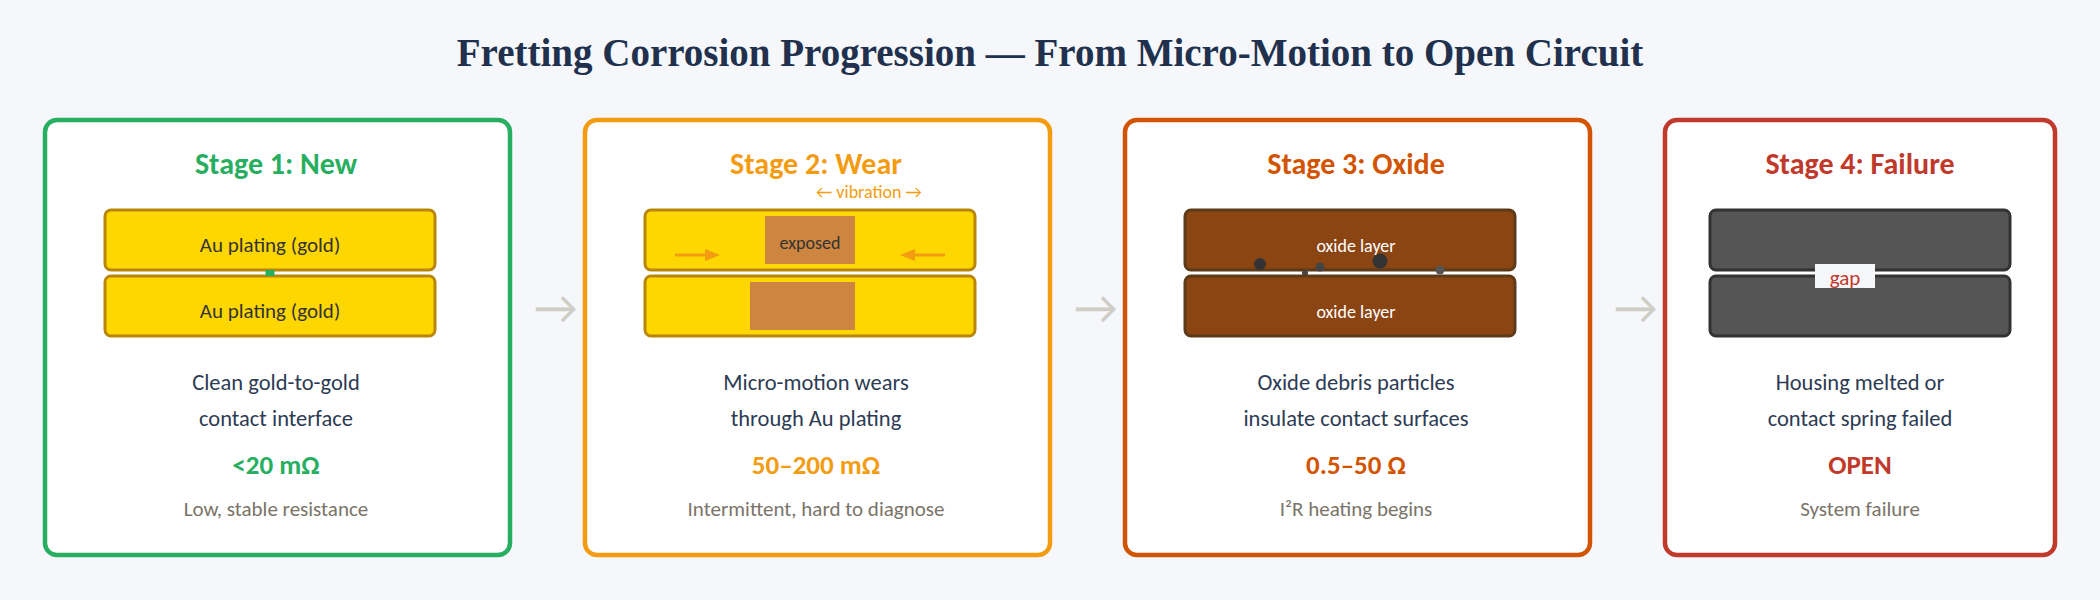
\includegraphics[width=\textwidth]{master_figs/fig7_fretting_progression.png}
\caption{Fretting corrosion progression, from clean gold-plated contacts through oxide accumulation to open-circuit failure. Note resistance escalation across stages.}
\label{fig:fretting_progression}
\end{figure}

Figure~\ref{fig:fretting_progression} illustrates the four-stage progression of fretting corrosion\index{fretting corrosion}.  At Stage~1, clean gold-plated contacts exhibit stable resistance below 20\,m$\Omega$. Vibration-induced micro-motion gradually wears through the plating at Stage~2, intermittently exposing base metal and raising resistance to 50--200\,m$\Omega$, often misdiagnosed as a ``loose connection.'' By Stage~3, accumulated oxide debris insulates the contact surfaces, resistance climbs to the ohm range, and $I^2R$ heating accelerates further degradation. Stage~4 is outright failure: melted housing, collapsed contact springs, or open circuit. Because Stage~2 symptoms are intermittent and position-dependent, fretting often passes bench-top continuity checks only to fail under dynamic load, a pattern students must learn to recognize.

\subsubsection{Overheating ($I^2 R$ Heating)}

\textbf{Mechanism}: Exceeding the current rating causes resistive heating at the contact interface. Heat accumulates in the housing, softening thermoplastic materials and potentially igniting adjacent insulation or components.

\textbf{Mitigations}:
\begin{itemize}[nosep,leftmargin=1.5em]
  \item Never exceed rated current; derate for ambient temperature.
  \item Select contacts with lower resistance (gold plating, larger cross-section).
  \item Distribute high currents across multiple contacts.
\end{itemize}

\subsubsection{Creep and Stress Relaxation}

\textbf{Mechanism}: Contact springs gradually lose their clamping force at elevated temperatures. The contact normal force decreases over time, increasing resistance and accelerating other failure modes.

\textbf{Mitigations}:
\begin{itemize}[nosep,leftmargin=1.5em]
  \item Specify beryllium copper (BeCu) contacts for any application above 60\,\degC{} continuous. BeCu resists creep far better than brass or phosphor bronze.
  \item Overspecify contact normal force for high-temperature applications.
\end{itemize}

\subsubsection{Moisture Ingress}

\textbf{Mechanism}: Water bridges between contacts, causing electrochemical corrosion, increased resistance, or direct short circuits.

\textbf{Mitigations}:
\begin{itemize}[nosep,leftmargin=1.5em]
  \item Specify appropriate IP rating per IEC~60529.
  \item Use sealed connectors with O-ring face seals and wire seals for any outdoor, vehicle, or washdown application.
  \item Apply conformal coating on exposed PCB connections.
\end{itemize}


% ══════════════════════════════════════════════════════════════════════
\section{Fluid System Connectors}
% ══════════════════════════════════════════════════════════════════════

\subsection{Threaded Pipe Fitting Standards}

Two incompatible tapered thread standards dominate global pipe fitting. Geography determines which you encounter.

\subsubsection{NPT\index{NPT thread}: National Pipe Taper (ASME B1.20.1)}

\begin{itemize}[leftmargin=1.5em]
  \item \textbf{Thread angle}: \ang{60} with pointed crests and roots.
  \item \textbf{Taper}: 1:16 (\textonequarter\,inch per inch of thread length, equivalent to \textthreequarters\,inch per foot).
  \item \textbf{Sealing mechanism}: Thread interference creates a metal-to-metal wedge seal. Because the thread form has clearance at crests and roots, NPT joints \emph{always} require supplemental sealing; either PTFE (Teflon) tape or anaerobic pipe dope.
  \item \textbf{NPTF variant}: ``Dryseal'' NPT uses a modified thread form with tighter root/crest tolerances that crushes metal at the interface, theoretically sealing without sealant. In practice, sealant is still recommended.
  \item \textbf{Size range}: 1/8\,in.\ to 24\,in.\ nominal pipe size (NPS).
  \item \textbf{Pressure rating}: Up to 15000\,psi depending on material and size.
  \item \textbf{Geography}: Dominant in the United States and Canada.
\end{itemize}

\subsubsection{BSP\index{BSP thread}: British Standard Pipe (ISO 228 / ISO 7-1)}

\begin{itemize}[leftmargin=1.5em]
  \item \textbf{Thread angle}: \ang{55} Whitworth form with rounded crests and roots.
  \item \textbf{Two sub-types}:
  \begin{itemize}[nosep]
    \item \textbf{BSPT} (designation ``R''): Tapered threads, seals like NPT via thread interference plus sealant.
    \item \textbf{BSPP} (designation ``G''): Parallel (straight) threads that \emph{do not} seal on the threads. Sealing is achieved with a bonded washer or O-ring compressed against a flat face.
  \end{itemize}
  \item \textbf{Size range}: 1/8\,in.\ to 6\,in.\ (inch-denominated but used globally outside North America).
  \item \textbf{Pressure rating}: Up to 6000\,psi typical.
  \item \textbf{Geography}: Dominant in Europe, Asia, and most of the world outside North America.
\begin{warningbox}[The Point of No Return: Thread Galling\index{thread galling}]
NPT threads are tapered at \ang{60}. BSP threads are tapered at \ang{55}. A \ang{55} BSP fitting \emph{will} start threading into a \ang{60} NPT port, and then seize. In stainless steel, this produces \textbf{galling}: a cold-weld that permanently fuses the two components. Both parts become scrap metal. There is no recovery.

\textbf{The Finger Test}: before applying any wrench, thread the fitting by hand. If you cannot achieve at least \textbf{three full turns by finger pressure alone}, STOP. The threads are incompatible, cross-threaded, or contaminated. Any attempt to force the connection with a wrench will result in irreversible damage. Verify the thread standard (NPT vs.\ BSP), clean both threads, apply appropriate sealant (Teflon tape for NPT, bonded washer for BSP parallel), and try again.
\end{warningbox}
\end{itemize}


\begin{warningbox}[Thread Galling: The Point of No Return]
In stainless steel or aluminum, forcing a mismatched or cross-threaded fitting with a wrench causes \textbf{galling}; a cold-weld that permanently destroys both components. Once galling begins, reaching for a bigger wrench turns a \$50 component into a \$100 mistake (two destroyed parts plus the replacement).

\textbf{The Finger Test}: if you cannot thread a fitting at least three full turns by hand, \textbf{STOP}. You are either cross-threaded or mixing thread standards. No amount of force or sealant can fix galled threads.

\textbf{Prevention for stainless-on-stainless connections}: apply nickel-based anti-seize compound (e.g., Permatex Nickel Anti-Seize or Loctite LB 8023) to the male threads before assembly. Anti-seize reduces friction and prevents the metal-to-metal adhesion that initiates galling. This is mandatory for any stainless steel fluid fitting in your design.
\end{warningbox}

\begin{warningbox}[Critical Incompatibility]
NPT (\ang{60} pointed threads) and BSP (\ang{55} rounded threads) are \textbf{NOT} interchangeable. They may appear to engage for a few turns but will not seal properly. Cross-threading causes galling, thread damage, and leaks that may develop catastrophically under pressure. \textbf{Always} verify thread standard with a thread pitch gauge before assembly.
\end{warningbox}

\begin{table}[htbp]
\centering
\small
\begin{tabularx}{\textwidth}{l X X}
  \toprule
  \textbf{Feature} & \textbf{NPT (ASME B1.20.1)} & \textbf{BSP (ISO 228 / ISO 7-1)} \\
  \midrule
  Thread angle & \ang{60}, pointed crests/roots & \ang{55} Whitworth, rounded crests/roots \\
  Taper & 1:16 (all NPT tapered) & BSPT tapered; BSPP parallel \\
  Sealing & Thread interference + sealant & BSPT: thread + sealant; BSPP: washer/O-ring \\
  Geography & U.S., Canada & Europe, Asia, rest of world \\
  Max pressure & 15000\,psi & 6000\,psi typical \\
  \bottomrule
\end{tabularx}
\caption{NPT vs.\ BSP thread comparison.}
\end{table}

\begin{figure}[htbp]
\centering
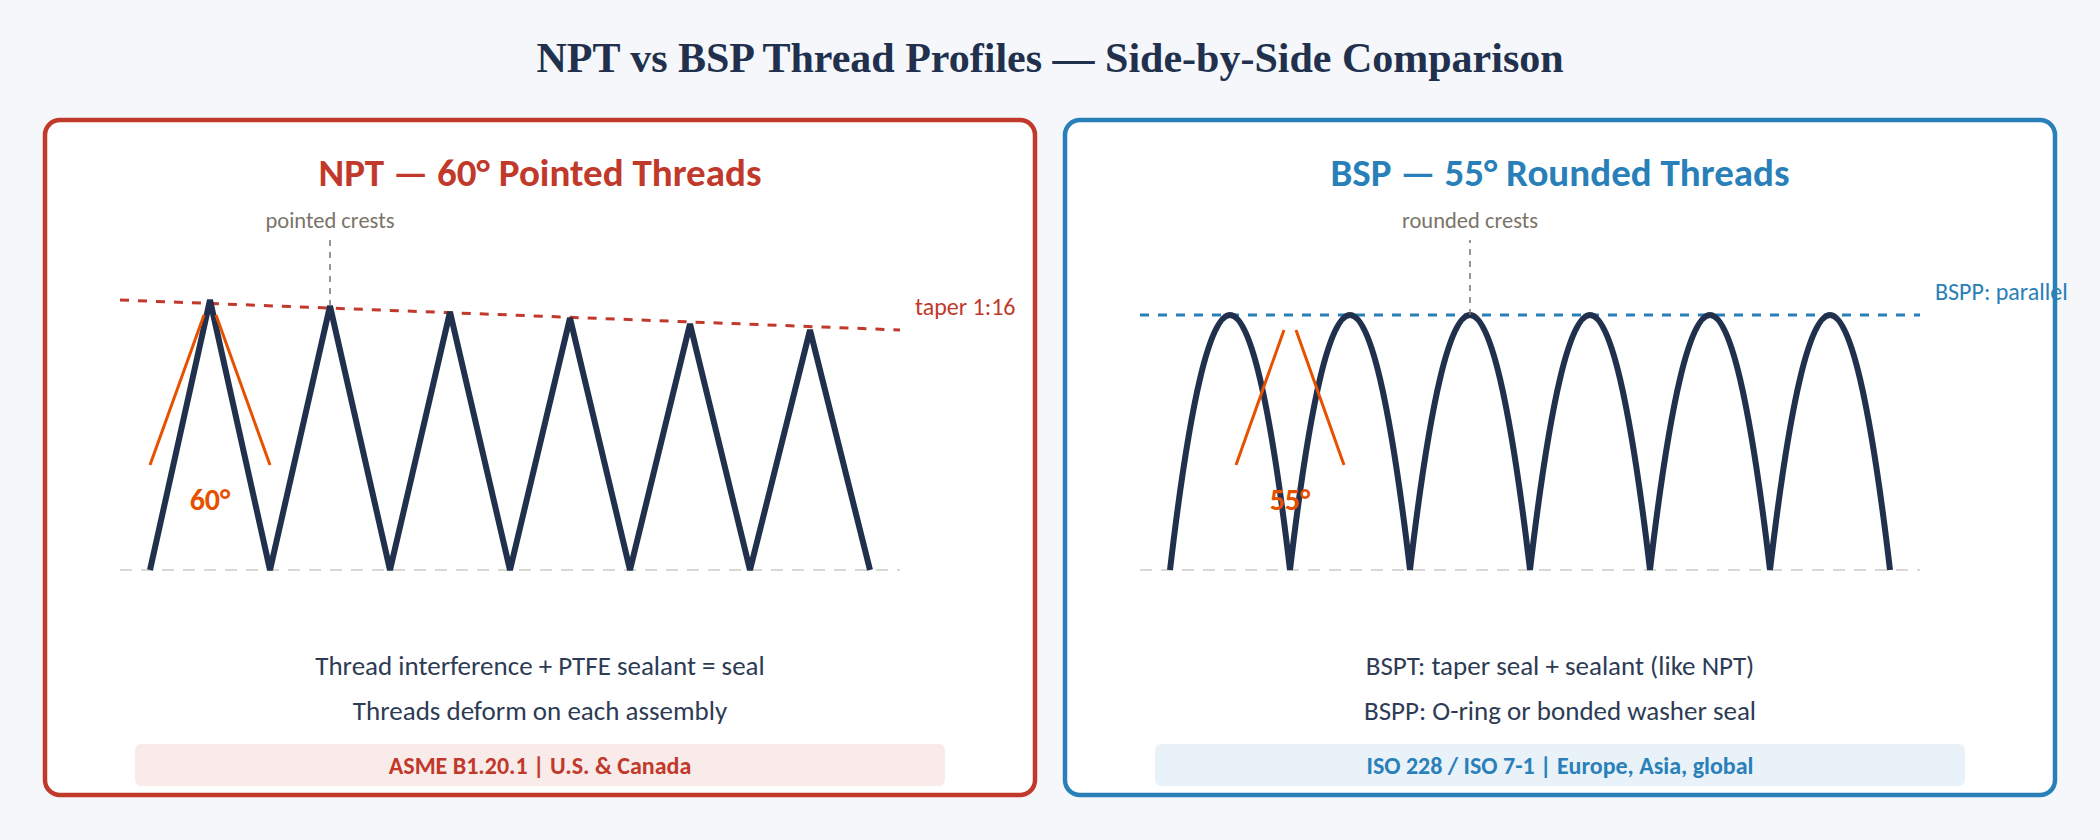
\includegraphics[width=\textwidth]{master_figs/fig5_thread_profiles.png}
\caption{NPT vs.\ BSP thread profiles; note the pointed \ang{60} crests on NPT versus the rounded \ang{55} Whitworth crests on BSP. These subtle geometric differences make the two standards completely incompatible.}
\label{fig:thread_profiles}
\end{figure}

Figure~\ref{fig:thread_profiles} places the two thread forms side by side so the geometric distinction is immediately visible. NPT's \ang{60} pointed crests create a wedging action as the taper engages; metal deforms at each assembly, which is why PTFE sealant is required and why each reassembly cycle slightly degrades the thread. BSP's \ang{55} Whitworth form uses rounded crests that are less prone to galling but follow an entirely different pitch schedule. The BSPP (parallel) variant does not seal on the thread at all; the thread merely provides clamping force while an O-ring or bonded washer creates the pressure boundary against a flat face. This is a critical distinction: applying PTFE tape to a BSPP fitting is a common student mistake that serves no purpose and can actually prevent proper washer compression.


\subsection{Tube Fittings and Quick-Connect Couplings}

Unlike threaded pipe fittings (which connect pipes), tube fittings connect \emph{tubing}; a product specified by outside diameter (OD) and wall thickness\index{wall thickness (injection molding)}, with tighter dimensional tolerances than pipe.

\subsubsection{JIC 37$^{\circ}$\ Flare (SAE J514)}

The tube end is flared to a \ang{37} cone that mates with a matching seat in the fitting body. The joint seals metal-to-metal; no sealant, tape, or elastomeric seal is required. The fitting uses a straight (non-tapered) thread; the thread provides clamping force only and does not contribute to sealing.

\begin{itemize}[nosep,leftmargin=1.5em]
  \item Reassemblable without degradation (unlike taper threads which deform with each assembly).
  \item The hydraulic industry standard worldwide.
  \item Pressure ratings to 10000\,psi.
  \item AN (Army--Navy) fittings are the military equivalent of JIC, with identical \ang{37} geometry.
\end{itemize}

\subsubsection{Compression Fittings (Swagelok-type)}

One or two ferrules (metal rings) are swaged (compressed) onto the tube OD when the nut is tightened. The ferrule bites into the tube, creating both a grip and a seal.

\begin{itemize}[nosep,leftmargin=1.5em]
  \item No welding, brazing, flaring, or special tools required.
  \item Tube OD is the sizing basis (1/4\,in., 3/8\,in., 1/2\,in., etc.).
  \item \textbf{Gaugeable}: Many designs include a visual indicator (gap gauge) so you can verify proper assembly by inspection.
  \item Pressure ratings up to 20000\,psi for medium-pressure configurations.
  \item Brands: Swagelok, Parker CPI/A-LOK, Ham-Let.
\end{itemize}

\subsubsection{Push-to-Connect}

The tube pushes into the fitting body. An internal collet (toothed ring) grips the tube OD, and an O-ring provides the seal. Assembly is one-handed and tool-free.

\begin{itemize}[nosep,leftmargin=1.5em]
  \item Common in pneumatics (air systems), typically up to $\sim$250\,psi.
  \item Common brands: SMC, Festo, John Guest.
  \item Fast assembly but limited to lower pressures and non-critical sealing applications.
\end{itemize}

\subsubsection{Quick-Disconnect (QD) Couplings}

Two halves, a plug and a socket, connect and disconnect by hand, often with a locking sleeve or collar. Self-sealing valves in one or both halves prevent fluid loss on disconnect.

\begin{itemize}[nosep,leftmargin=1.5em]
  \item \textbf{Flat-face}: Minimal fluid spillage on disconnect, used in clean or environmentally sensitive applications.
  \item \textbf{Poppet-valve}: Spring-loaded valve seals on disconnect, less expensive but more spillage.
  \item Common applications: hydraulic tool circuits, coolant loops, test equipment.
\end{itemize}

\begin{table}[htbp]
\centering
\small
\begin{tabularx}{\textwidth}{l c c X}
  \toprule
  \textbf{Fitting Family} & \textbf{Pressure} & \textbf{Seal Type} & \textbf{Key Characteristic} \\
  \midrule
  JIC 37$^{\circ}$\ Flare & 10000\,psi & Metal-to-metal & Reassemblable; hydraulic standard \\
  Compression & 20000\,psi & Ferrule swage & No special tools; gaugeable \\
  Push-to-Connect & 250\,psi & O-ring & Tool-free; pneumatics \\
  Quick-Disconnect & Varies & Valve + O-ring & Hand-connect; self-sealing \\
  \bottomrule
\end{tabularx}
\caption{Tube fitting and coupling comparison.}
\end{table}

\begin{figure}[htbp]
\centering

\includegraphics[width=\textwidth]{master_figs/fig3_fluid_connectors.png}
\caption{Four major fluid connector families with thread standards, pressure ratings, and sealing mechanisms.}
\label{fig:fluid_connectors}
\end{figure}

\begin{figure}[htbp]
\centering
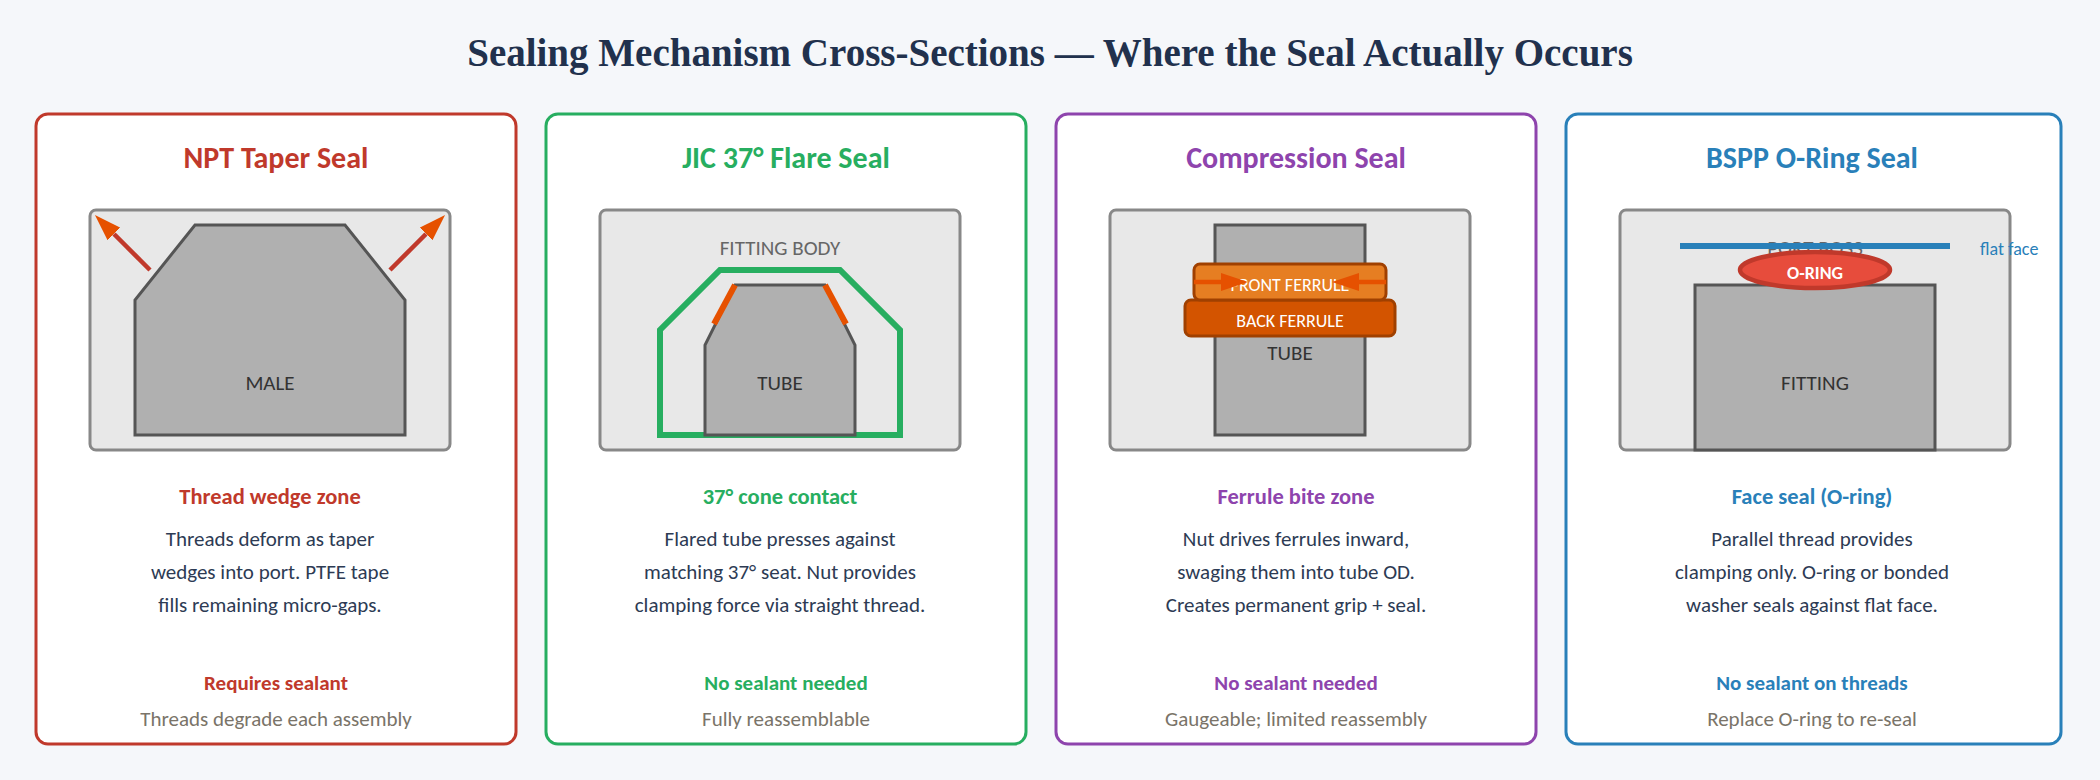
\includegraphics[width=\textwidth]{master_figs/fig6_seal_cross_sections.png}
\caption{Sealing mechanism cross-sections showing exactly where each seal forms: NPT thread wedge, JIC \ang{37} flare cone contact, compression ferrule bite zone, and BSPP face-seal O-ring.}
\label{fig:seal_cross_sections}
\end{figure}

Figure~\ref{fig:seal_cross_sections} shows the internal geometry of each sealing method so students can visualize \emph{why} proper torque and assembly procedures matter. In the NPT taper seal, the thread flanks themselves deform to create a pressure boundary, which is why sealant is mandatory to fill the remaining micro-gaps and why repeated assembly progressively damages the seal surfaces. In the JIC \ang{37} flare, the cone-shaped tube end presses against a matching seat in the fitting body; the straight thread provides clamping force only. This metal-to-metal geometry is fully reassemblable because the sealing surfaces do not deform. In compression fittings, the front ferrule bites radially into the tube OD while the back ferrule provides axial grip; the nut drives both ferrules during initial makeup. Once swaged, the ferrule is permanently deformed, which limits reassembly. In the BSPP face seal, the parallel thread clamps the fitting against the port face while an O-ring in a groove creates the pressure boundary, the thread contributes zero sealing.


\subsection{Key Fluid Connector Specifications}
\label{sec:fluidspecs}

When specifying a fluid connector in your design documentation, define each of the following.

\subsubsection{Working Pressure}

The maximum continuous operating pressure (psi or bar). Always specify \emph{working} pressure, not burst pressure. Standard safety factors:
\begin{itemize}[nosep,leftmargin=1.5em]
  \item Hydraulic: burst $\geq 4\times$ working.
  \item Pneumatic: burst $\geq 3\times$ working.
  \item \textbf{Design rule}: Never operate above 25\% of burst pressure.
\end{itemize}

\subsubsection{Temperature Range}

Temperature determines seal material selection:

\begin{table}[htbp]
\centering
\small
\begin{tabularx}{\textwidth}{l c X}
  \toprule
  \textbf{Seal Material} & \textbf{Range} & \textbf{Notes} \\
  \midrule
  Buna-N (Nitrile, NBR) & $-40$ to 250\,$^{\circ}$F & General purpose; petroleum-compatible \\
  Viton (FKM) & $-20$ to 400\,$^{\circ}$F & Chemical resistance; fuel systems \\
  PTFE (Teflon) & $-100$ to 500\,$^{\circ}$F & Widest range; chemically inert; no elasticity \\
  EPDM & $-65$ to 300\,$^{\circ}$F & Steam/water service; not oil-compatible \\
  \bottomrule
\end{tabularx}
\caption{Seal material temperature ranges and applications.}
\end{table}

Always verify seal compatibility with both the fluid \emph{and} the operating temperature.

\subsubsection{Fluid Compatibility}

Verify fitting body material and seal material against the working fluid using manufacturer chemical compatibility charts:
\begin{itemize}[nosep,leftmargin=1.5em]
  \item \textbf{Stainless steel}: Resists most chemicals; highest cost.
  \item \textbf{Brass}: Common for water, air, and general service; not for ammonia or acetylene.
  \item \textbf{Carbon steel}: Standard for hydraulic oil systems; requires corrosion protection.
\end{itemize}

\subsubsection{Thread / Tube Size}

\begin{itemize}[nosep,leftmargin=1.5em]
  \item \textbf{Threaded fittings}: Specified by Nominal Pipe Size (NPS). Note that NPS does \emph{not} equal the actual outside diameter. For example, 1/2\,in.\ NPS pipe has an OD of 0.840\,in.
  \item \textbf{Tube fittings}: Specified by tube outside diameter (OD). Common sizes: 1/4\,in., 3/8\,in., 1/2\,in.
  \item \textbf{Always measure with calipers and thread gauges}. Never assume a size by visual inspection.
\end{itemize}

\subsubsection{End Configuration}

Select the geometry that connects the fitting to your system: straight, elbow (45$^{\circ}$\ or 90$^{\circ}$), tee, cross, union, reducer, or bulkhead. 

\begin{tipbox}[Minimize Joints]
Every fitting joint is a potential leak point. Design your routing to minimize the total number of fittings in a line. Avoid stacking street elbows in series; use a single 90$^{\circ}$\ elbow or a pre-bent tube run instead.
\end{tipbox}


\subsection{Fluid Connector Failure Modes}
\label{sec:fluidfailure}

\subsubsection{Cross-Threading}

\textbf{Mechanism}: Attempting to mate NPT into BSP (or vice versa), or even same-standard threads started at an angle, destroys thread profiles and causes immediate or delayed leaks.

\textbf{Mitigations}:
\begin{itemize}[nosep,leftmargin=1.5em]
  \item Always verify thread standard with a thread pitch gauge before assembly.
  \item Start threads by hand for at least two full turns before applying a wrench.
  \item NPT: \ang{60} pointed threads. BSP: \ang{55} rounded threads. They \emph{feel} similar but are not compatible.
\end{itemize}

\subsubsection{Over-Tightening}

\textbf{Mechanism}: Excessive torque cracks port bosses (especially aluminum and cast iron), deforms compression ferrules beyond recovery, and splits flare cones. Over-tightening destroys more fittings than under-tightening.

\textbf{Mitigations}:
\begin{itemize}[nosep,leftmargin=1.5em]
  \item Always use manufacturer-specified torque values.
  \item Use a calibrated torque wrench, not a ``feel'' wrench.
  \item For Swagelok-type fittings, follow the turns-past-finger-tight specification exactly.
\end{itemize}

\subsubsection{Seal Degradation}

\textbf{Mechanism}: O-rings and gaskets deteriorate from chemical attack (incompatible fluid), UV exposure, thermal cycling, and simple age. Seals swell, harden, crack, or take a permanent compression set.

\textbf{Mitigations}:
\begin{itemize}[nosep,leftmargin=1.5em]
  \item Establish replacement intervals based on seal material and service conditions.
  \item Keep spare seal kits on hand.
  \item Verify seal material compatibility with the fluid and temperature range before installation.
\end{itemize}

\subsubsection{Vibration Fatigue}

\textbf{Mechanism}: Cyclic stress at tube-to-fitting junctions nucleates fatigue cracks. Under pressure, these cracks propagate to failure; potentially a sudden, high-pressure fluid release.

\textbf{Mitigations}:
\begin{itemize}[nosep,leftmargin=1.5em]
  \item Use proper tube support clamps spaced per manufacturer recommendations.
  \item Route tubing to avoid sharp bends and unsupported cantilever lengths.
  \item Include flexible hose segments at vibration sources (pumps, engines).
\end{itemize}

\begin{warningbox}[High-Pressure Fluid Injection Injury]
A hydraulic line leak may be invisible; a pinhole stream at 2000\,psi can penetrate skin and inject fluid deep into tissue, causing catastrophic damage that requires emergency surgery within hours. \textbf{Never} check for hydraulic leaks by running a bare hand along a pressurized line. Use a piece of cardboard or a thermal camera instead. This is one of the most serious and least-understood hazards in hydraulic system work, and students designing or testing any pressurized fluid system must be explicitly aware of it before commissioning.
\end{warningbox}


% ══════════════════════════════════════════════════════════════════════
\section{Selection and Design Practice}
% ══════════════════════════════════════════════════════════════════════

\subsection{Connector Selection Logic}

Whether electrical or fluid, connector selection follows a universal logic sequence:

\begin{enumerate}[leftmargin=1.5em]
  \item \textbf{Rating}: What current, voltage, pressure, or flow must it handle?
  \item \textbf{Environment}: Temperature range, vibration, moisture/IP, chemical exposure?
  \item \textbf{Serviceability}: How often must it be connected/disconnected? What tools are available?
  \item \textbf{Cost}: What is the budget per connection, including tooling?
  \item \textbf{Standards}: Which industry/regulatory standards apply (IEC, SAE, ASME, MIL)?
  \item \textbf{Space}: What are the physical envelope constraints?
\end{enumerate}

\begin{figure}[htbp]
\centering

\includegraphics[width=\textwidth]{master_figs/fig4_selection_framework.png}
\caption{Decision tree for electrical and fluid connector selection.}
\label{fig:selection_framework}
\end{figure}

\begin{tipbox}[Spec the Connector First]
The connector determines wire gauge, tube OD, termination tooling, and housing envelope. Select the connector family first (based on rating, environment, and serviceability), then design the wiring or tubing around it, not the other way around.
\end{tipbox}

\subsection{Design Rules of Thumb}

\begin{enumerate}[leftmargin=1.5em]
  \item \textbf{Derate everything.} Never operate at 100\% of rated current, pressure, or temperature. A 25\% safety margin is minimum engineering practice; 50\% is professional practice for critical systems.

  \item \textbf{Design for Assembly\index{Design for Assembly (DFA)} (DFA).} Provide wrench clearance around fittings. Group fluid connections for leak-test access. Use consistent connector families within a subsystem to reduce tool count and spare parts inventory.

  \item \textbf{For fluid systems}: Verify thread standard with a gauge before assembly. Use manufacturer torque specifications. Pressure-test every joint before commissioning; hydrostatic test at $1.5\times$ working pressure per ASME B31.3.

  \item \textbf{For electrical systems}: Pull-test a sample of crimps per IPC/WHMA-A-620. Verify contact resistance with a milliohm meter. Document every connector in your wire harness schedule.

  \item \textbf{Document every choice.} Record part number, manufacturer, specifications, and selection rationale in your Bill of Materials (BOM). Your future self and your teammates will need this information for procurement, assembly, and troubleshooting.
\end{enumerate}


\subsection{Key Standards Reference}

\begin{longtable}{l l p{7.5cm}}
  \toprule
  \textbf{Standard} & \textbf{Org} & \textbf{Scope} \\
  \midrule
  \endfirsthead
  \toprule
  \textbf{Standard} & \textbf{Org} & \textbf{Scope} \\
  \midrule
  \endhead
  IEC 61984~[2] & IEC & Electrical connector safety requirements, testing, and performance criteria \\
  IEC 60529~[3] & IEC & IP ingress protection rating system (IP67, IP68, IP69K) \\
  MIL-DTL-38999 & U.S.\ DoD & Military circular connectors for high-performance, harsh-environment applications \\
  UL 486A-486B & UL & Safety certification for wire connectors: crimp, solder, and IDC terminations \\
  SAE J514 & SAE & JIC 37$^{\circ}$\ flare hydraulic tube fittings; dimensions and performance requirements \\
  ASME B1.20.1 & ASME & NPT tapered pipe thread form, dimensions, and tolerances \\
  ISO 228 / ISO 7-1 & ISO & BSP parallel (BSPP) and tapered (BSPT) pipe thread standards \\
  ASME B31.3 & ASME & Process piping code; materials, fabrication, inspection, and testing \\
  \bottomrule
\end{longtable}


% ══════════════════════════════════════════════════════════════════════
\section{Applying Connectors in Your Design Projects}
% ══════════════════════════════════════════════════════════════════════

Incorrect connector selection is one of the most common failure modes in student design projects. The following workflow ensures systematic coverage.

\begin{enumerate}[leftmargin=1.5em]
  \item \textbf{Create a connection schedule early.} List every electrical and fluid joint in your design. Classify each by type (wire-to-wire, wire-to-board, NPT, JIC, etc.). This becomes a living document through your design reviews.

  \item \textbf{For every electrical connection, specify}: connector family, pin count, current rating (derated), voltage rating, IP rating, termination method, wire gauge, and mating cycles.

  \item \textbf{For every fluid connection, specify}: fitting standard (NPT, BSP, JIC, or compression), nominal size, working pressure, seal material, fluid compatibility, and assembly torque.

  \item \textbf{Build a complete BOM} with manufacturer part numbers and procurement sources. Recommended suppliers:
  \begin{itemize}[nosep]
    \item Electrical: Digi-Key, Mouser, Newark, Allied.
    \item Fluid: Swagelok, Parker, McMaster-Carr, Grainger.
  \end{itemize}

  \item \textbf{Design review milestones}:
  \begin{itemize}[nosep]
    \item \textbf{PDR}: Present your connection schedule.
    \item \textbf{CDR}: Present datasheets and torque specifications.
    \item \textbf{FDR}: Demonstrate assembly procedures and test results.
  \end{itemize}

  \item \textbf{Test every connection before commissioning}: Pull-test electrical crimps, measure contact resistance with a milliohm meter, and pressure-test all fluid joints at $1.5\times$ working pressure.
\end{enumerate}


% ══════════════════════════════════════════════════════════════════════
\section{Quick-Reference Summary}
% ══════════════════════════════════════════════════════════════════════

\begin{keyconceptbox}[Five Key Takeaways]
\begin{enumerate}[nosep,leftmargin=1.5em]
  \item Electrical connectors are classified by \emph{what they connect} (wire-to-wire, wire-to-board, board-to-board) and \emph{how they terminate} (crimp, solder, IDC, screw, press-fit).
  \item For every electrical connection, specify: current rating, voltage rating, IP rating, contact resistance, and mating cycles, and derate for temperature.
  \item Fluid connectors require matching thread standards. NPT $\neq$ BSP. JIC 37$^{\circ}$\ flare and compression fittings avoid the pitfalls of tapered-thread sealing.
  \item Failure modes differ by domain: electrical joints fail from fretting corrosion and $I^2R$ overheating; fluid joints fail from cross-threading and seal degradation.
  \item Every connector specification follows the same logic: \textbf{rating $\to$ environment $\to$ serviceability $\to$ cost $\to$ standards $\to$ space}. Document everything in your BOM.
\end{enumerate}
\end{keyconceptbox}


% ══════════════════════════════════════════════════════════════════════
\section{Artifact Handoff: What This Chapter Supports}
\begin{table}[htbp]\centering\small
\begin{tabularx}{\textwidth}{l X l}
\toprule
\textbf{Artifact} & \textbf{Description} & \textbf{Forward Reference} \\
\midrule
Connector Specifications & Selected connectors with ratings in BOM & Ch.~5 (ICDs) \\
Wire/Tube Routing & Harness design and fluid line layout & Assembly drawings \\
\bottomrule
\end{tabularx}
\end{table}


\begin{keyconceptbox}[Requirements Mapping: From Connector Specs to Shall-Statements]
Connector specifications generate system requirements:
\begin{itemize}[nosep,leftmargin=1.5em]
\item ``Outdoor deployment in rain'' $\to$ SYS-REQ: All external connectors shall be rated IP67 or higher.
\item ``Field-replaceable sensor'' $\to$ SYS-REQ: Sensor connections shall use keyed, tool-free connectors rated for $\geq$100 mating cycles.
\item ``Motor draws 8\,A continuous'' $\to$ CONN-REQ: Motor power connectors shall be rated for $\geq$10\,A continuous (20\% margin) with 12\,AWG wire termination.
\item ``Hydraulic test pressure 200\,psi'' $\to$ CONN-REQ: All fluid fittings shall be rated for $\geq$800\,psi working pressure ($4\times$ safety factor per hydraulic standard).
\end{itemize}
Every connector in your BOM must trace to a requirement. If you cannot write a shall-statement for it, you have not justified the selection.
\end{keyconceptbox}

\begin{quickrefbox}[Quick Reference: Common Connector Families]
\begin{table}[H]\centering\small
\begin{tabularx}{\linewidth}{l c c c X}
\toprule
\textbf{Family} & \textbf{Current} & \textbf{Voltage} & \textbf{Pitch} & \textbf{Typical Use} \\
\midrule
JST-PH & 2\,A & 100\,V & 2.0\,mm & LiPo batteries, small sensors \\
JST-XH & 3\,A & 250\,V & 2.5\,mm & Battery packs, board-to-wire \\
Molex KK & 4\,A & 250\,V & 2.54\,mm & General board-to-wire, fans \\
Molex Micro-Fit & 8.5\,A & 600\,V & 3.0\,mm & Motor power, high-current \\
Dupont/0.1'' & 3\,A & 250\,V & 2.54\,mm & Breadboard jumpers, headers \\
USB-C & 3--5\,A & 5--20\,V & --- & Data + power, standard interface \\
Barrel jack & 5\,A & 12--24\,V & --- & Wall adapters, bench supplies \\
XT60 & 60\,A & 500\,V & --- & High-current battery, motors \\
Anderson PP & 15--45\,A & 600\,V & --- & EV battery, solar, high-power \\
Deutsch DT & 13\,A & 500\,V & --- & Automotive, harsh environment \\
\bottomrule
\end{tabularx}
\end{table}
\end{quickrefbox}

\section{Practice Questions for Quiz Preparation}
% ══════════════════════════════════════════════════════════════════════

Use these questions to test your understanding. Answers follow on the next page.

\subsection{Conceptual Questions}

\begin{enumerate}[leftmargin=1.5em]
  \item What are the three fundamental elements of every electrical connector?

  \item A connector is rated at 15\,A per contact at 25\,\degC{}. Your design has an ambient temperature of 75\,\degC{} and all 12 contacts are loaded. Why should you \emph{not} assume 15\,A per contact is safe?

  \item Explain why fretting corrosion is considered the ``most insidious'' electrical connector failure mode.

  \item You need to connect a hydraulic line rated at 5000\,psi that will be disconnected for maintenance monthly. Which fitting family is most appropriate? Why?

  \item A colleague suggests using PTFE tape on a BSPP fitting. Is this correct? Explain.

  \item What is the difference between rated working voltage and dielectric withstand voltage? Which should appear in your design documentation?

  \item Why does NPS (Nominal Pipe Size) create confusion when specifying fittings?

  \item Describe two mitigations for vibration fatigue in fluid tubing systems.

  \item You measure 50\,m$\Omega$ contact resistance on a connector carrying 8\,A. How much power is dissipated as heat at that contact? Is this a concern?

  \item Compare the sealing mechanisms of NPT, JIC 37$^{\circ}$\ flare, and compression fittings. Which requires sealant?
\end{enumerate}

\subsection{Application / Scenario Questions}

\begin{enumerate}[resume,leftmargin=1.5em]
  \item Your design team is designing an outdoor weather station. You need a 6-pin connector for sensor signals (all under 500\,mA) that will be installed once and never disconnected. What IP rating, plating, and mating-cycle specification would you select? Justify your choices.

  \item A pneumatic system in your project uses 1/4\,in.\ OD nylon tubing at 80\,psi. Recommend a fitting type and explain why.

  \item Your design uses both NPT and BSP components (sourced from U.S.\ and European manufacturers). What steps must you take to ensure safe assembly?

  \item You are specifying connectors for a cooling loop carrying a 50/50 ethylene glycol--water mix at 200\,$^{\circ}$F and 50\,psi. What seal material would you select? What body material?

  \item At your CDR, a reviewer asks: ``How did you verify your crimp terminations are reliable?'' Describe the test procedure you would reference.

  \item \textbf{Diagnostic scenario}: Your team's prototype passes a low-voltage continuity check on the bench (all connections show $<$1\,$\Omega$), but the system experiences intermittent sensor dropouts and a motor controller that occasionally faults when the prototype is running on a vibration table or driving over rough terrain. Where do you start your investigation, and what failure modes should you suspect? Describe the diagnostic steps you would take, referencing at least three concepts from this module.
\end{enumerate}


\newpage
\subsection{Answers}

\begin{enumerate}[leftmargin=1.5em]
  \item Contacts (conductive pins/sockets), housing (insulating body), and termination (wire-to-contact joint).

  \item Two derating effects compound: (a) elevated ambient temperature reduces the thermal headroom of the housing, and (b) thermal stacking from all 12 contacts being loaded raises the internal housing temperature further. The manufacturer's derating curve must be consulted; actual safe current per contact could be as low as 10\,A or less.

  \item Fretting corrosion develops slowly from micro-vibration, manifests as intermittent (not permanent) high resistance, is invisible without disassembly, and is difficult to reproduce during troubleshooting. By the time symptoms are consistent, oxide debris has accumulated extensively.

  \item JIC 37$^{\circ}$\ flare (SAE J514). It handles 10000\,psi (well above 5000\,psi), provides a metal-to-metal seal that doesn't degrade with reassembly, and is designed for repeated disconnect/reconnect without special tools beyond standard wrenches. Compression would also work but ferrules deform on initial assembly, making reassembly less reliable.

  \item Incorrect. BSPP (G-type) uses parallel threads that do \emph{not} seal on the threads. Sealing is achieved with a bonded washer or O-ring against a flat face. PTFE tape is used on \emph{tapered} threads (NPT, BSPT) where the thread interference provides the primary seal. Applying tape to BSPP serves no useful purpose and may prevent proper washer compression.

  \item Working voltage is the maximum voltage at which the connector is rated for continuous, safe operation, including creepage and clearance margins per IEC 61984. Dielectric withstand (breakdown) voltage is the voltage at which insulation fails; it is a destructive test limit, not an operating specification. Always specify working voltage in design documentation.

  \item NPS is a nominal designation, not a physical dimension. For example, 1/2\,in.\ NPS has an OD of 0.840\,in. Engineers unfamiliar with this convention may attempt to match fittings by measuring OD, leading to incorrect specifications. Always reference the NPS table and verify with thread gauges.

  \item (a) Install tube support clamps at manufacturer-recommended intervals to eliminate unsupported spans. (b) Include flexible hose segments at vibration sources (pumps, engines) to decouple cyclic motion from rigid tubing.

  \item $P = I^2R = (8)^2 \times 0.050 = 3.2\,W$. Yes, this is a concern; 3.2\,W of localized heat will raise the contact and housing temperature significantly. This level of contact resistance suggests degraded contacts that should be inspected and potentially replaced.

  \item NPT: Thread interference creates a wedge seal, but clearance at crests/roots requires supplemental sealant (PTFE tape or pipe dope). JIC 37$^{\circ}$: Metal-to-metal cone seal at the flared tube end; no sealant required. Compression: Ferrule swaged onto tube OD creates the seal mechanically; no sealant required. Only NPT (and BSPT) requires sealant.

  \item IP67 (dust-tight, survives 1\,m immersion for rain/flooding protection). Gold plating (resists corrosion in outdoor environment with humidity and temperature cycling). 25--50 mating cycles (permanent installation, only disconnected for rare maintenance). Lower mating cycle connectors are less expensive and can be more robust.

  \item Push-to-connect fittings. At 80\,psi with nylon tubing, this is well within the 250\,psi range of push-to-connect. Benefits: tool-free assembly, compatible with nylon tubing, easy reconfiguration, and widely available in 1/4\,in.\ OD size from SMC, Festo, or John Guest.

  \item (a) Create a thread identification chart for the project listing which ports are NPT and which are BSP. (b) Verify every connection with a thread pitch gauge (\ang{60} = NPT, \ang{55} = BSP) before assembly. (c) If adaptation is needed, use NPT-to-BSP adapter fittings from a reputable manufacturer. Never force-thread. (d) Label all ports on your assembly drawings with thread standard.

  \item Seal: Viton (FKM); compatible with ethylene glycol, rated to 400\,$^{\circ}$F (above the 200\,$^{\circ}$F operating temperature). Body: stainless steel or brass (both compatible with glycol--water). Avoid carbon steel unless corrosion-protected, as glycol solutions can be mildly corrosive to unprotected ferrous metals.

  \item Reference IPC/WHMA-A-620 standard. Procedure: (a) Pull-test a statistical sample of crimps at the specified force for the wire gauge and contact size. (b) Cross-section a sample crimp to verify the cold-weld zone under magnification. (c) Measure contact resistance across each mated pair with a milliohm meter; verify $<$20\,m$\Omega$ for gold-plated contacts. (d) Document results with crimp force values, pass/fail criteria, and inspector sign-off.

  \item This scenario synthesizes three interconnected failure modes. \textbf{Primary suspect: fretting corrosion.} The hallmark is a system that passes static bench testing but fails under dynamic load, exactly the intermittent, vibration-dependent behavior described in the fretting progression (Section~\ref{sec:elecfailure}, Figure~\ref{fig:fretting_progression}). Diagnostic steps: (a)~Measure contact resistance across every mated connector pair with a milliohm meter \emph{while the system is subject to vibration} (tap on connectors, flex cables). Resistance that fluctuates from milliohms to ohms on disturbance confirms fretting. (b)~Check for $I^2R$ heating: use a thermal camera to identify hot connectors under load. A connector running 10\,A through a fretting contact at 500\,m$\Omega$ dissipates 5\,W, enough to soften a nylon housing. (c)~Inspect strain relief: if cables transmit vehicle vibration directly to the contact zone, fretting is accelerated regardless of plating. (d)~Check connector specifications: are tin-plated contacts being used in a high-vibration application where gold plating is warranted? Is the contact normal force sufficient? (e)~For the motor controller faults specifically, consider whether the power connector is derated for the actual ambient temperature inside the enclosure under operation. Resolution: replace affected contacts with gold-plated equivalents, add proper strain-relief clamps, install secondary locking features (CPA clips), and retest under dynamic load with milliohm monitoring.
\end{enumerate}


% ══════════════════════════════════════════════════════════════════════


\subsection{Application Scenario Answers}
\begin{enumerate}[leftmargin=1.5em, start=11]
\item \textbf{Redesigning a student project from soldered connections to connectors}:

\textbf{Step 1}: Identify every wire-to-wire and wire-to-board connection in the system. Create a connection table: source, destination, signal type (power/signal/data), current, voltage, mating cycles expected.

\textbf{Step 2}: Group connections by subsystem boundary. Each subsystem-to-subsystem boundary gets one multi-pin connector (e.g., sensor module connects to controller via one 4-pin JST-XH: VCC, GND, SDA, SCL).

\textbf{Step 3}: Select connector families. For low-current signals ($<$1\,A): JST-XH (wire-to-board, 2.5\,mm pitch, rated 3\,A, keyed). For power ($>$1\,A): XT30 (rated 30\,A, gendered, compact) or Anderson Powerpole (genderless, stackable). For board-to-board: standard 2.54\,mm pin headers with locking housings.

\textbf{Step 4}: Create a wiring diagram showing every connector with pin assignments, wire colors, and wire gauges. This diagram is a CDR deliverable.

\textbf{Step 5}: Label every connector pair with matching alphanumeric codes (J1/P1, J2/P2, etc.) on both the connector and the wiring diagram.

Benefits: any subsystem can be disconnected, tested independently, and reconnected. Failed modules can be swapped without soldering. The system can be disassembled for transport and reassembled on-site.
\end{enumerate}

